
\documentclass[preprint,12pt]{elsarticle}

\usepackage[spanish]{babel}
\usepackage{amssymb}
\usepackage{graphicx}
\usepackage{lineno}
\usepackage[utf8]{inputenc}
\usepackage{url}
\usepackage{natbib} 
\usepackage{amsmath} 
\usepackage{amssymb} 
\usepackage{float}

\begin{document}
	
	\begin{frontmatter} 

		\title{\huge INFORME DE LABORATORIO 09 INSTALACIÓN Y GESTION DE UNA BASE DE DATOS MONGODB}
		
		\author{Huichi Contreras, Franklin Carlos         	(2016054948)} 
		\address{Escuela Profesional de Ingeniería de Sistemas}
		\address{Universidad Privada de Tacna}
		\address{Tacna, Perú}
		

	\end{frontmatter}

%% INTRODUCION ----------------------------------------------------------------------------------------------------------------

\section{INFORMACIÓN GENERAL} 

\subsection {\textbf{Objetivos}}
\begin{itemize}
	\item Instalación y gestion de una base de datos MongoDB
\end{itemize}

\subsection {\textbf{Equipos, materiales, programas y recursos utilizados}}
\begin{itemize}
	\item Computadora con sistema operativo Windows XP, Vista, Windows 7, Windows 8 y/o Windows 8.1.
	\item CPU SLAT-capable feature al menos 4GB de RAM
	\item Docker Desktop (Para lo cual se debe primero crear una cuenta en Docker Hub)
	\item Studio 3T
	\item Documento JSON
	\item ISO MongoDB
\end{itemize}

%% ----------------------------------------------------------------------------------------------------------------------------------


%% MARCO TEÓRICO ------------------------------------------------------------------------------------------------------------

\section{Marco Teórico}

%% PRIMERA SUBSECCION 

\subsection {\textbf{Docker}}
Docker se define como un proyecto de código abierto que proporciona una capa de abstracción y virtualización a nivel de sistema operativo, a través de la instalación de contenedores de software.

\subsection {\textbf{MongoDB}}
MongoDB (del inglés humongous, enorme) es un sistema de base de datos NoSQL orientado a documentos de código abierto.\\
En lugar de guardar los datos en tablas, tal y como se hace en las bases de datos relacionales, MongoDB guarda estructuras de datos BSON (una especificación similar a JSON) con un esquema dinámico, haciendo que la integración de los datos en ciertas aplicaciones sea más fácil y rápida.

\section{PROCEDIMIENTO}

\subsubsection{\textbf{Paso 1: Instalar imagen de mongodb}}
\begin{figure}[H]
	\begin{center}
		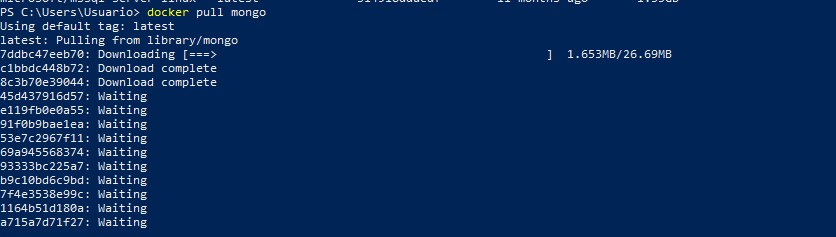
\includegraphics[width=12cm]{./IMAGENES/foto1} 
		\caption{Descargar imagen de mongoDB}
	\end{center}
\end{figure}

\begin{figure}[H]
	\begin{center}
		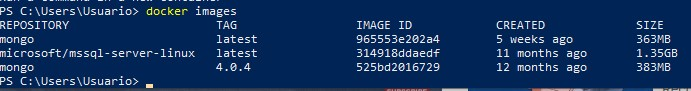
\includegraphics[width=12cm]{./IMAGENES/foto2} 
		\caption{Imagenes que tenemos descargadas entre ellas mongoDB}
	\end{center}
\end{figure}

\begin{figure}[H]
	\begin{center}
		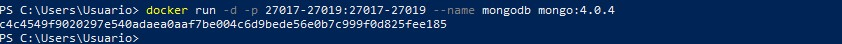
\includegraphics[width=12cm]{./IMAGENES/foto3} 
		\caption{Creamos un contenedor de MongoDB}
	\end{center}
\end{figure}

\begin{figure}[H]
	\begin{center}
		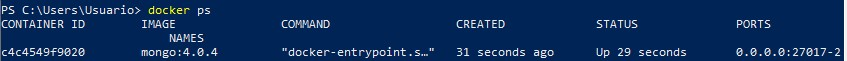
\includegraphics[width=12cm]{./IMAGENES/foto4} 
		\caption{Comoporbamos quese halla creado el contenedor}
	\end{center}
\end{figure}

\subsubsection{\textbf{Paso 2: Gestionar mongoDB desde mi contenedor}}

\begin{figure}[H]
	\begin{center}
		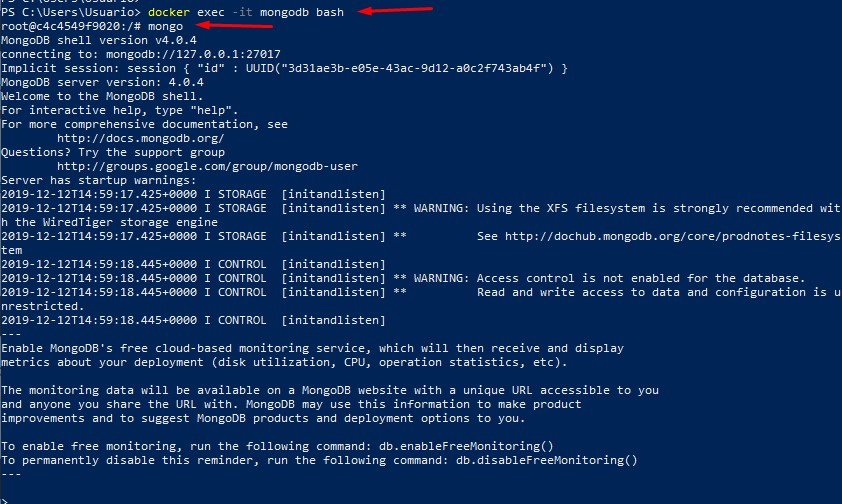
\includegraphics[width=12cm]{./IMAGENES/foto5} 
		\caption{Ejecutamos el Shell de MongoDB}
	\end{center}
\end{figure}


\begin{figure}[H]
	\begin{center}
		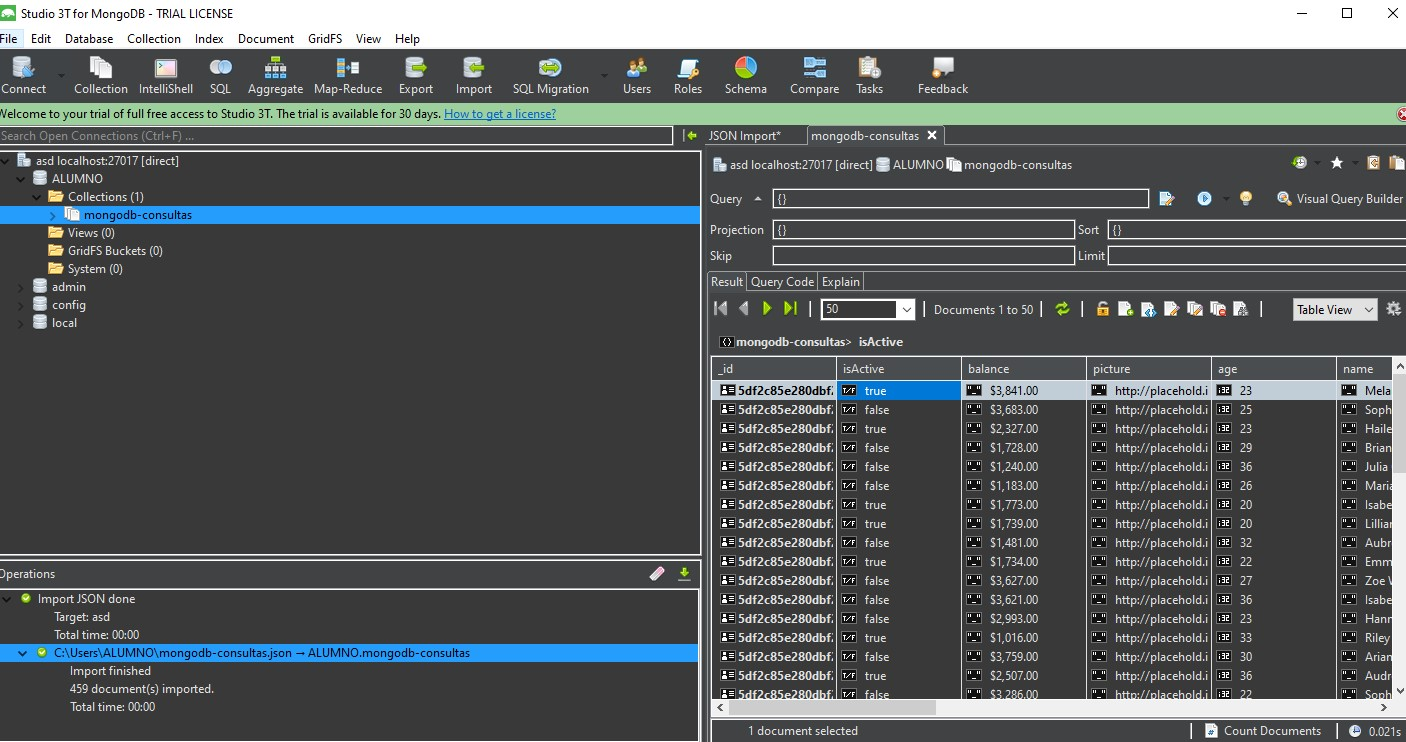
\includegraphics[width=12cm]{./IMAGENES/foto6} 
		\caption{Para importar datos utilizaremos el software Studio 3T}
	\end{center}
\end{figure}

\subsubsection{\textbf{Paso 3: Consultas con la base de datos MongoDb}}

\begin{figure}[H]
	\begin{center}
		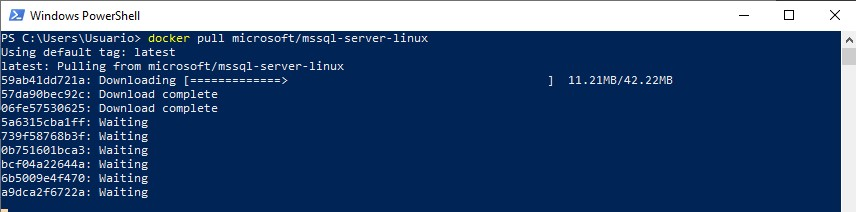
\includegraphics[width=07cm]{./IMAGENES/foto7} 
		\caption{Mostramos las bases de datos creadas}
	\end{center}
\end{figure}

\begin{figure}[H]
	\begin{center}
		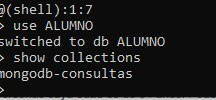
\includegraphics[width=07cm]{./IMAGENES/foto8} 
		\caption{Usaremos la base de datos llamada Alumnos}
	\end{center}
\end{figure}

\begin{figure}[H]
	\begin{center}
		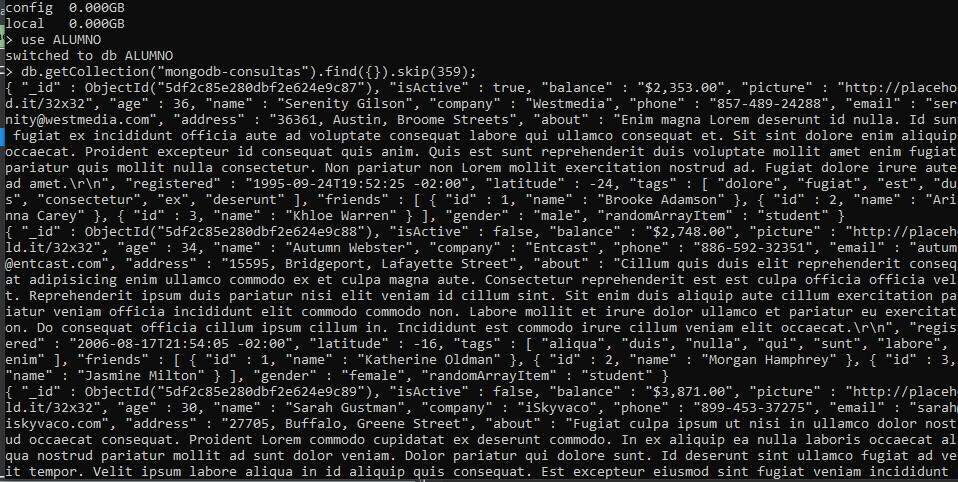
\includegraphics[width=12cm]{./IMAGENES/foto9} 
		\caption{Ingresamos el siguiente comando: db.getCollection( 'mongodb-consultas' ).find().skip(359)}
	\end{center}
\end{figure}

\begin{figure}[H]
	\begin{center}
		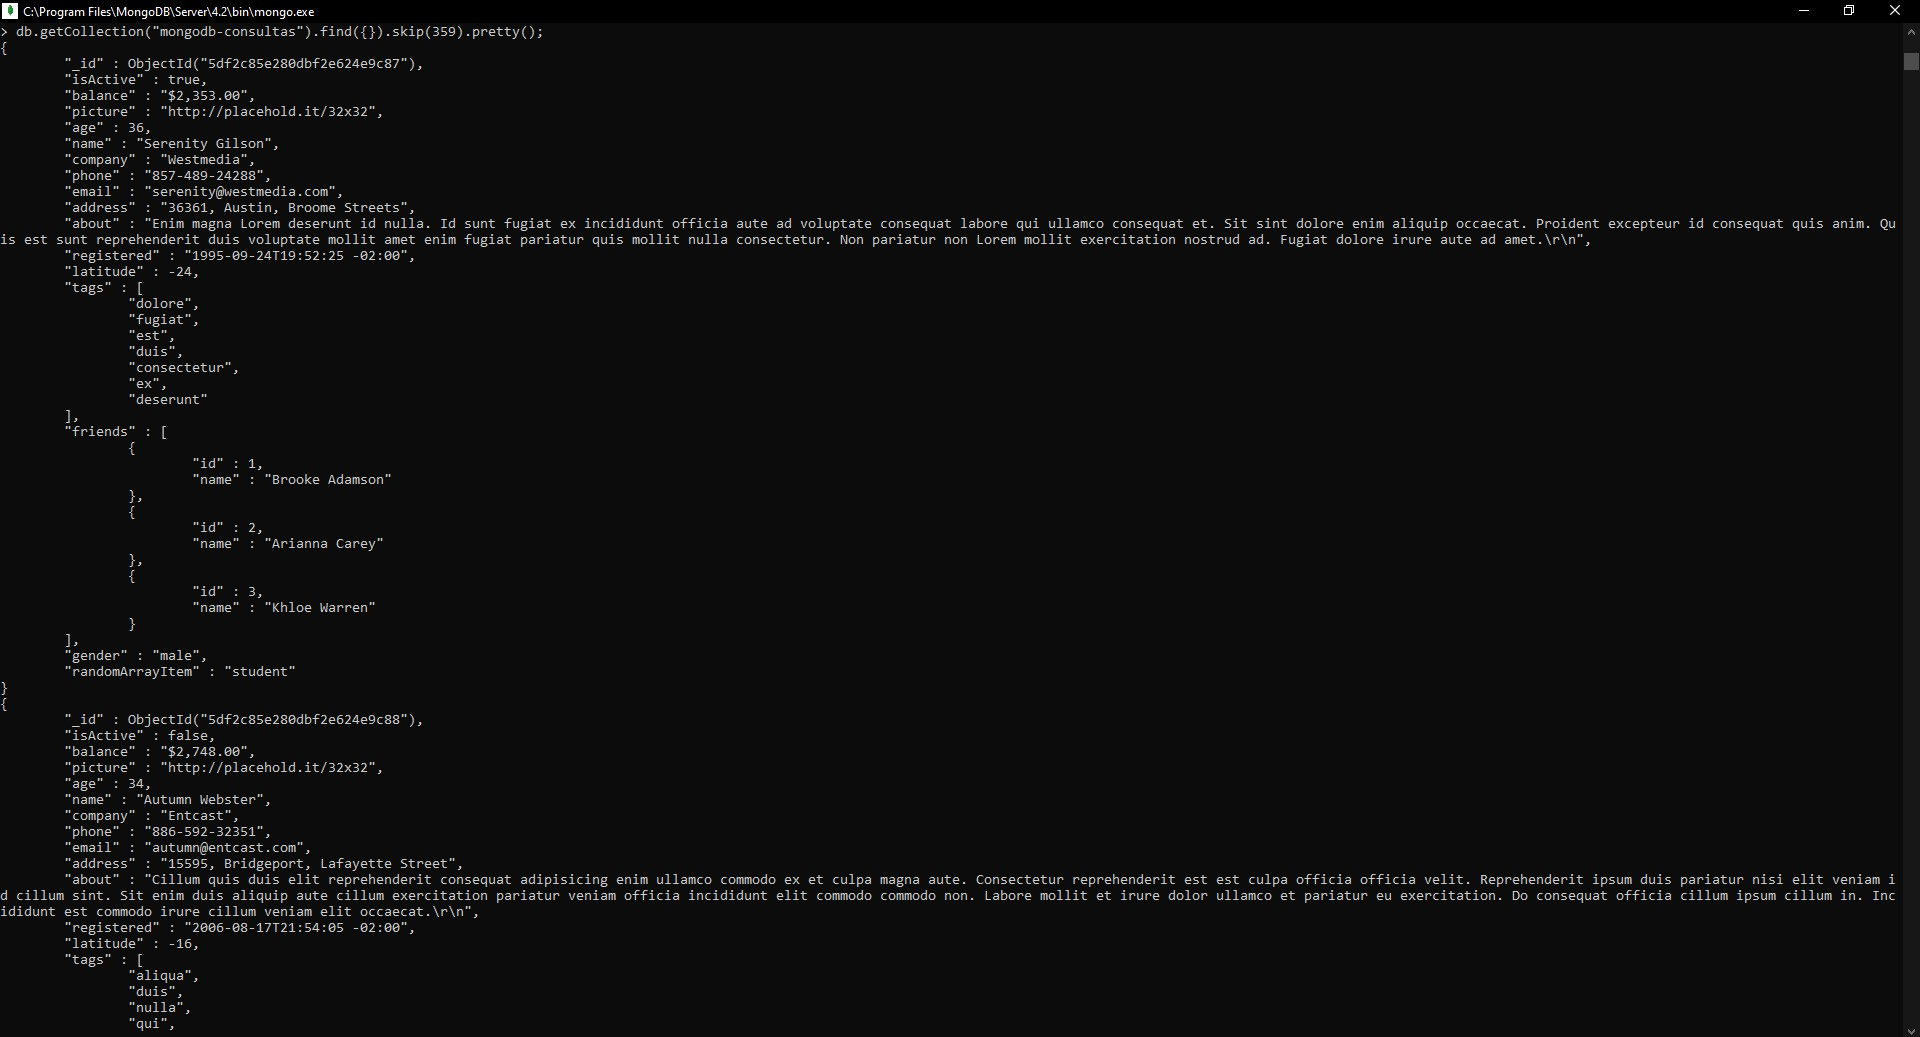
\includegraphics[width=12cm]{./IMAGENES/foto10} 
		\caption{Ingresamos el siguiente comando: db.getCollection( 'mongodb-consultas' ).find().skip(359).pretty()}
	\end{center}
\end{figure}

\begin{figure}[H]
	\begin{center}
		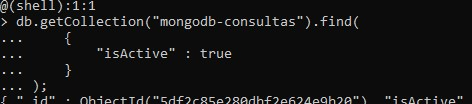
\includegraphics[width=12cm]{./IMAGENES/foto11} 
		\caption{Ahora verificaremos los campos que esten en estado activo con el siguiente comando: db.getCollection( 'mongodb-consultas' ).find( 'isActive' : true ); }
	\end{center}
\end{figure}

\begin{figure}[H]
	\begin{center}
		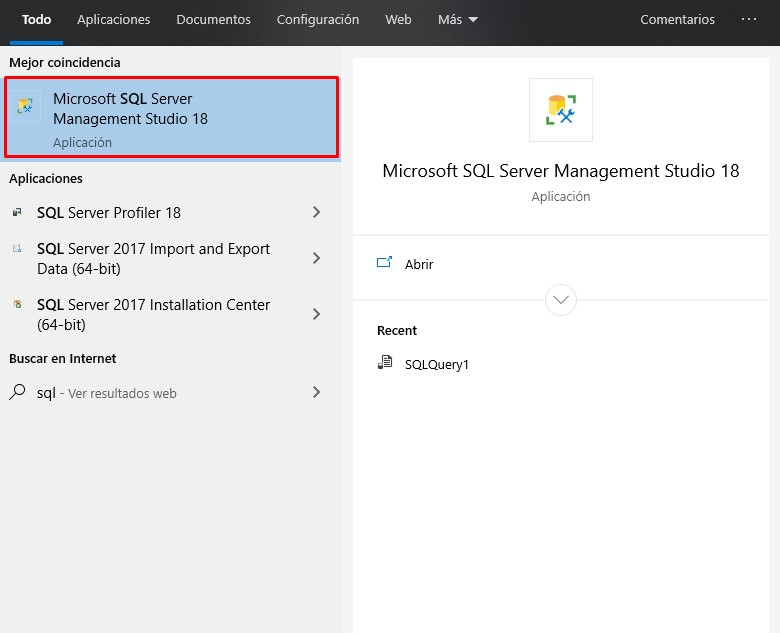
\includegraphics[width=12cm]{./IMAGENES/foto12} 
		\caption{Vemos los resultados de la consulta anterior}
	\end{center}
\end{figure}

\section{ANALISIS E INTERPRETACION DE RESULTADOS }
\begin{itemize}
	\item ¿Qué indican los resultados? \\
	Pudimos realizar exitosamente la conexión de nuestro contenedor a la base de datos
	\item ¿Que se ha encontrado?\\
	Encontré una manera más rápida de poder realizar consultas mediante NoSQL Mongo DB mediante una importacion desde un archivo JSON.
\end{itemize}


\section{CONCLUSION}
En conclusión, Las bases de datos NoSQL son una tecnología muy potente y variada que, si se sabe
emplear de forma correcta, resulta ser una herramienta valiosísima que permitirá
almacenar grandes cantidades de datos y extraer conocimiento de ellos de forma
eficiente, tan necesario hoy en día debido al fenómeno BigData. No en vano, los puestos
profesionales de informáticos que poseen conocimientos sobre alguna de estas
tecnologías se están comenzando a demandar ampliamente

\end{document}
